\documentclass[12pt]{article}
\usepackage[francais]{babel}%\usepackage[english]{babel}
\usepackage{amsmath,amsthm,amscd}\usepackage{amssymb,verbatim,amssymb}
\usepackage{amsfonts,amscd, graphicx, dsfont}

\usepackage{remreset}
\makeatletter\@removefromreset{footnote}{chapter}\makeatother 
\usepackage{mathrsfs}  
\usepackage[top=20mm, bottom=22mm, left=23mm, right=24mm]{geometry}
\numberwithin{equation}{section}
\theoremstyle{plain}
\newenvironment{changemargin}[2]{\begin{list}{}{%
\setlength{\topsep}{0pt}%
\setlength{\leftmargin}{0pt}%
\setlength{\rightmargin}{0pt}%
\setlength{\listparindent}{\parindent}%
\setlength{\itemindent}{\parindent}%
\setlength{\parsep}{0pt plus 1pt}%
\addtolength{\leftmargin}{#1}%
\addtolength{\rightmargin}{#2}%
}\item }{\end{list}}


\newtheorem{thm}{Theorem}[section]
\newtheorem{prop}{Proposition}[section]
\newtheorem{lem}{Lemma}[section]
\newtheorem{defn}{Definition}[section]
\newtheorem{cor}{Corollary}[section]
\newtheorem{rem}{Remark}
\newtheorem{ex}{Example}
\def\i1{\mathds{1}}
\def\h1{\hspace{0.2cm}}
\def\v1{\vskip0.2cm}
\def\no{\noindent}
\def\txt{\text}
\def\it{\textit}
\def\bf{\textbf}
\def\R{\mathbb{R}}
\def\Z{\mathbb{Z}}
\def\N{\mathbb{N}}
\def\C{\mathbb{C}}
\def\P{\mathbb{P}}
\def\E{\mathbb{E}}
\def\I{\mathbb{I}}
\def\D{\mathbb{D}}
\def\a{\alpha}
\def\b{\beta}
\def\g{\gamma}
\def\d{\delta}
\def\e{\varepsilon}
\def\k{\kappa}
\def\f{\varphi}
\def\z{\zeta}
\def\t{\theta} 
\def\l{\lambda}
\def\m{\mu}
\def\n{\nu}
\def\s{\sigma}
\def\x{\textbf{x}}
\def\el{\ell}
\def\itun{\item[\textit{1.}]}
\def\itdeux{\item[\textit{2.}]}
\def\ittrois{\item[\textit{3.}]}
\def\ite{\item[$(e)$]}
\def\ita{\item[$(a)$]}
\def\itb{\item[$(b)$]}
\def\itc{\item[$(c)$]}
\def\itd{\item[$(d)$]}
\def\ite{\item[$(e)$]}
\def\iti{\item[$(i)$]}
\def\itii{\item[$(ii)$]}
\def\itiii{\item[$(iii)$]}
\def\itiv{\item[$(iv)$]}
\def\itv{\item[$(v)$]}
\def\cA{\mathcal{A}}
\def\cB{\mathcal{B}}
\def\cC{\mathcal{C}}
\def\cD{\mathcal{D}}
\def\cE{\mathcal{E}}
\def\cF{\mathcal{F}}
\def\cG{\mathcal{G}}
\def\cH{\mathcal{H}}
\def\cI{\mathcal{I}}
\def\cJ{\mathcal{J}}
\def\cK{\mathcal{K}}
\def\cL{\mathcal{L}}
\def\cM{\mathcal{M}}
\def\cN{\mathcal{N}}
\def\cO{\mathcal{O}}
\def\cP{\mathcal{P}}
\def\cQ{\mathcal{Q}}
\def\cR{\mathcal{R}}
\def\cS{\mathcal{S}}
\def\cT{\mathcal{T}}
\def\cU{\mathcal{U}}
\def\cV{\mathcal{V}}
\def\cW{\mathcal{W}}
\def\cX{\mathcal{X}}
\def\cY{\mathcal{Y}}
\def\cZ{\mathcal{Z}}
\def\sA{{\mathscr A}}
\def\sB{{\mathscr B}}
\def\sC{{\mathscr C}}
\def\sD{{\mathscr D}}
\def\sE{{\mathscr E}}
\def\sF{{\mathscr F}}
\def\sG{{\mathscr G}}
\def\sH{{\mathscr H}}
\def\sI{{\mathscr I}}
\def\sJ{{\mathscr J}}
\def\sK{{\mathscr K}}
\def\sL{{\mathscr L}}
\def\sM{{\mathscr M}}
\def\sN{{\mathscr N}}
\def\sO{{\mathscr O}}
\def\sP{{\mathscr P}}
\def\sQ{{\mathscr Q}}
\def\sR{{\mathscr R}}
\def\sS{{\mathscr S}}
\def\sT{{\mathscr T}}
\def\sU{{\mathscr U}}
\def\sV{{\mathscr V}}
\def\sW{{\mathscr W}}
\def\sX{{\mathscr X}}
\def\sY{{\mathscr Y}}
\def\sZ{{\mathscr Z}}
\def\gb{\overline{\gamma}}
\def\no{\noindent}
\def\eq{\eqalign}
\def\ss{\smallskip}
\def\ms{\medskip}
\def\bs{\bigskip}
\def\q{\quad}
\def\qq{\qquad}
\usepackage{color}
\usepackage{float}

\def\hb{\hbox}
\def\cvfd{\h1{\overset{(d)}\longrightarrow \h1}}%convergence en lois fini dimentionnel
\def\cvp{\h1{\overset{\P}\longrightarrow \h1}}% convergence en prob
\def\cvl{\h1{\overset{\cL}\longrightarrow \h1}}% convergence en loi
\def\eqfd{\h1{\overset{(d)}= \h1}}
%equalité en loi finis dimentionnelle
\def\L{\Lambda}
\usepackage{python}

\newcommand{\abs}[1]{\lvert#1\rvert}
\title{}


\begin{document}

\begin{center}
\begin{figure}

\includegraphics[width=18cm]{images} 
\end{figure}
\begin{center}{\Huge\textbf{Projet Big Data : k-means Clustering}\v1
 \texttt{20 janvier 2020}
}\vskip1cm
\begin{center}
Salem Amenallah,  \footnote{amenallah.salem@dauphine.tn
/ id cluster de Dauphine: \textbf{user81}
} Gaidi Mohamed Amine \footnote{mohamedamine.gaidi@dauphine.tn / id cluster de Dauphine : \textbf{user 83}
} \& Aziz ben ammar \footnote{. aziz.benammar@dauphine.tn / id cluster de Dauphine : \textbf{user74}
}\v1
Université Paris-Dauphine $|$ Tunis


\end{center}

\end{center}
\end{center}


%%%%%%%%%%%%%%%%%%%%%%%%%%%%

%%%%%%%%%%%%%%%%%%%%%%%%%%%%%

\tableofcontents
%\maketitle
\newpage

%{\color{blue}   }
%black	noir
%white	blanc
%red	rouge
%green	vert
%blue	bleu
%cyan	cyan
%magenta	magenta
%yellow	jaune


%\tableofcontents
%%%%%%%%%%%%%%%%%%%%%%%%%%%%%%%%%%%%%%%%%%%%%%%%

\section{Introduction}
Le problème du partitionnement d'un ensemble de données (\textit{data clustering}) non labelisé en groupes (ou clusters) apparait  dans une grande variété d'applications (à voir le lien suivant pour quelques applications des algorithmes de clustering  \color{blue}https://datafloq.com/read/7-innovative-uses-of-clustering-algorithms/6224\color{black} ).
L'un des algorithmes de clustering les plus connus et les plus utilisés est l'algorithme de  \textit{k-means} [1]. \v1
La popularité de k-means est due principalement à sa simplicité (le seul paramètre qui doit être choisi est ($k= \text{le nombre des clusters souhaité}$), et aussi sa vitesse (plusieurs extensions de ce algorithmes ont été le but des travaux de recherche). \v1 
Dans ce contexte plusieurs efforts et articles scientifiques ont été réalisés pour améliorer la qualité des \textit{résultats} produit par k-means. Une telle tentative est l'algorithme k-means$++$, qui utilise la même méthode itérative mais une initialisation différente [2]. Cet algorithme a tendance à produire de meilleurs clusters dans la pratique, bien qu'il s'exécute parfois plus lentement en raison de l'étape d'initialisation supplémentaire. \v1
Compte tenu de l'omniprésence du clustering $k$-means et de ses variantes, il est naturel de se demander comment cet algorithme pourrait être adapté à un environnement distribué.
 Dans ce projet, nous montrons comment implémenter $k$-means et $k$-means$++$ en utilisant le framework MapReduce en utilisant Hadoop \& Spark. De plus, nous décrivons un autre algorithme MapReduction, $k$-means$++$, qui peuvent également être efficaces et terme de vitesse et simplicité sur un ensembles de données (Dataset) trés grande tout en implémentant ces algorithmes distribués dans Spark, les testons sur la dataset \texttt{Iris} et un autre grands ensembles de données du monde réel en rapportons et discutant les résultats.
\section{Premier pas avec  kmeans-dario-x.py \& iris.data.txt}
\no
La première étape consiste à téléchargez la Dataset Iris\\ {\color{blue} wget https://www.dropbox.com/s/9kits2euwawcsj0/iris.data.txt}\\ \no et la charger sur notre répertoire HDFS et vérifier qu'elle est bien enregistrer\\ {\color{blue} hdfs dfs -put 5000-8.txt /user/user81}.\\ 
{ \color{blue} hdfs dfs -ls /user/user81}.\\
Ensuite on télecharge notre fichier Python à optimiser \\
{\color{blue}wget https://www.dropbox.com/s/tm9lk6vffci5yzr/kmeans-dario-x.py}.\\
Finalement on lancer notre programme Python (kmeans-dario-x.py)  à partir du master node du cluster. en utilisan 
{\color{blue}spark-submit kmeans-dario-x.py}
On ajoute: \\
{\color{blue} import time \\
startTime = time.time()
} \\
puis dans la main function on ajoute\\
{\color{blue}print("Le temp d'exécution est \%s seconds ---" \% (time.time() - startTime))
}
 pour la vusualisation du temp d'éxécution du code.
\subsection{Notations:}
Dans ce qui suit, on utilisera les notations suivantes:
\begin{enumerate}
\item Soit les $x_i\in\R^d$, $i\in\{1,\ldots, n\}$ les observations que nous voulons partitionner.
\item $\mu_k \in\R^d, k\in\{1,\ldots , K\}$ sont des  moyennes où $\mu_k$ est le centre du cluster $k$. Nous allons
noté $\mu$ la matrice associée.
\item $z_i^k $ sont des variables indicatrices associées à $x_i$ telles que $z_i^k = $  si $x_i$ appartien au cluster $k$, et $z_i=$ sinon
\item $z$ est la matrice don't les composantes sont égaux à $z_i^k$
\end{enumerate}
Finalement en définie la déformation $$J(\mu , z )= \sum_{i=1}^{n}\sum_{k=1}^{K} z_i^k ||x_i - \mu_k||
^2$$
\subsection{Etapes de l'algorithme}
L'algorithme se décompose en quatres étapes principales : Aprés  
choisir $K$ points géolocalisés aléatoires comme centres de départ 
\v1\no
=============================================\\
k-means \\
=============================================
\begin{itemize}
\iti On chosit un vecteur $\mu$
\itii On trouve tous les points les plus proches de chaque centre (on affecte chaque point à son centroide le plus proche) i.e on minimuse $J$ par rapport à $z$ :  $z_i^k =1 si ||x_i - \mu_k ||^2 = \min_s ||x_i -\mu _s ||^2$
\itiii Trouvez le nouveau centre de chaque cluster (on recalcule les coordonnées des centroides de chaque cluster (en calculant la moyenne des coordonnées des points qui lui sont rattachés). i.e  on minimise $J$ par rapport à $\m_k =\frac{\sum_i s_i^k x_i} {\sum_i z_i^k}$ 
\itiv on refait l'etapes $(ii)$ et $(iii)$ en calculant les coordonnées des centroides de chaque cluster (en calculant
la moyenne des coordonnées des points qui lui sont rattachés), jusqu'à ce que la distance totale entre les points d'une itération et le suivant soit inférieure à la distance de convergence spécifiée ( i.e l'algorithme converge vers un optimum local).
\end{itemize}
\subsection{Analyse \& remarques}

On commence cette partie par une remarque trés importante qu'il Il y a un nombre fini de partitions possibles à $k$ clusters (classes ici dans le cas de la dataset Iris ). De plus, chaque étape de l'algorithme fait strictement diminuer la fonction de coût, positive, et fait découvrir une meilleure partition. Cela permet d'affirmer que l'algorithme converge toujours en temps fini.\v1 
Le critère de convergence pour l'étape $(iv)$ est généralement lorsque l'erreur totale cesse de changer entre les étapes, dans ce cas un minimum local de la fonction du cout est atteint. À $k$ fixé, la complexité lisse est polynomiale pour certaines configurations, dont des points dans un espace euclidien. Si $k$ fait partie de l'entrée, la complexité lisse est encore polynomiale pour le cas euclidien. Ces résultats expliquent en partie l'efficacité de l'algorithme en pratique.

\begin{rem}
Dans d'autres cas, certaines implémentations mettent fin à la recherche lorsque le changement d'erreur entre les itérations tombe en dessous d'un certain seuil. C'est pour cela on trouve dans des livres et des réferences que le partitionnement final n'est pas toujours optimal. et le temps de calcul peut-être exponentiel en fonction du nombre de vecteurs à classer, même dans le plan. Généralement (Dans la pratique) et aussi dans notre cas, on a imposer une limite sur le nombre d’itérations ou un critère sur l'amélioration entre itérations.
\end{rem}
\begin{rem}
En principe, le nombre d'itérations nécessaires pour que l'algorithme converge complètement peut être très
grand, mais sur des ensembles de données réels, l'algorithme converge généralement en au plus quelques dizaines d'itérations.
\end{rem}

\begin{figure}[H]
\centering
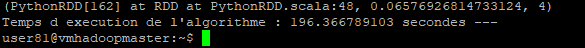
\includegraphics{temp1}
\caption{Le temps d'éxécution de kmeans-dario-x.py
}
\end{figure}

\section{Notre approche pour l'Optimisation: k-means $++$}
\color{blue} Code : kmeansProject.py \color{black}

L'algorithme est le suivant:
\subsection{Etapes de l'algorithme k-means $++$}
\v1\no
=============================================\\
k-means++ \\
=============================================

\begin{itemize}
\iti Choisissez la première moyenne $\mu_1$ \textbf{au hasard} dans l'ensemble $X=$ $\{x_1,\ldots, x_k\}$ et ajoutez-la à l'ensemble $M=\{\mu_1,\ldots, \mu_k\}$.
\itii Pour chaque point $x \in X$, calculez la distance au carré $D (x)$ entre $x$ et la moyenne la plus proche en $M$. 
\itiii Choisissez la prochaine moyenne au hasard dans l'ensemble $X$, où la probabilité qu'un point $x \in X$ soit choisi est proportionnelle à $D (x)$, et ajoutez à $M$.
\itiv Répétez les étapes (ii) et (iii) $ k - 1$ fois pour produire $k$ moyennes initiales.
\itv Appliquer l'algorithme k-means standard fournis dans la section 1, initialisé avec ces moyens
\end{itemize}

\subsection{Points faible de l'algorithme k-means-dario-x.py}
$\bullet$ Tout d'abord aprés le calcule du produit cartésien et pour accélérer le calcule on enlève la colone des classes des fleures par exemple 'Iris-setosa'. Par cette méthode en enlève une colonne de la boucle. Puis on la récupère aprés \texttt{assignment $=$ min\_dist.join(data)}\\
$\bullet$ Dans l'étape (ii) de k-means-dario-x.py au lieu d'affecte chaque point à son centroide le plus proche( opération faite pour chaque point) on calcule juste la distance $D (x)$ entre $x$ et la moyenne la plus proche dans $M$ et choisir la prochaine moyenne au (hasard), qui plus rapide en tèrme de complexité  
\subsection*{Analyse \& remarques}
Cet algorithme est conçu pour choisir un ensemble de moyens initiaux bien séparés les uns des autres. Dans l'article [2] où ils décrivent d'abord l'algorithme k- means $++$, les auteurs Arthur et Vassilvitskii le testent sur quelques ensembles de données du monde réel et démontrent qu'il conduit à des améliorations de l'erreur finale
sur l'algorithme k-means standard. Étant donné que chaque itération de cette initialisation prend du temps $O (|M|nd)$ et que la taille de $M$ augmente de 1 à chaque itération jusqu'à ce qu'elle atteigne $k$, la complexité totale de k-means ++ est $O (k^2 nd)$, plus $O (nkd)$ par itération une fois la  méthode k-means commence.

\section{Temps d'exécution \& output}


\begin{figure}[H]
\centering
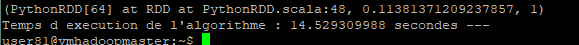
\includegraphics{temp_ex}
\caption{Le temps d'éxécution
}
\end{figure}

Et on a le meme output que kmeans-dario-x.py
\begin{figure}[H]
\centering
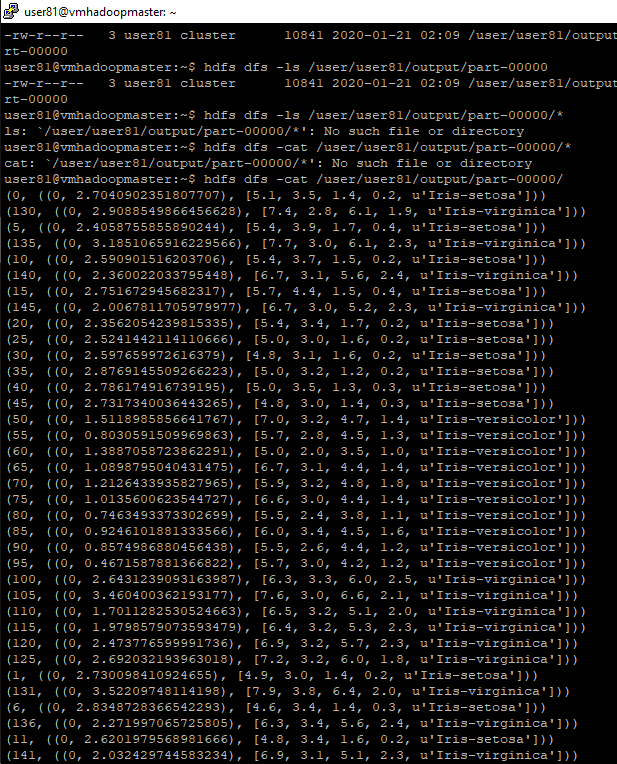
\includegraphics[width=10cm]{out1}
\caption{output Part 1
}
\end{figure}\begin{figure}[H]
\centering
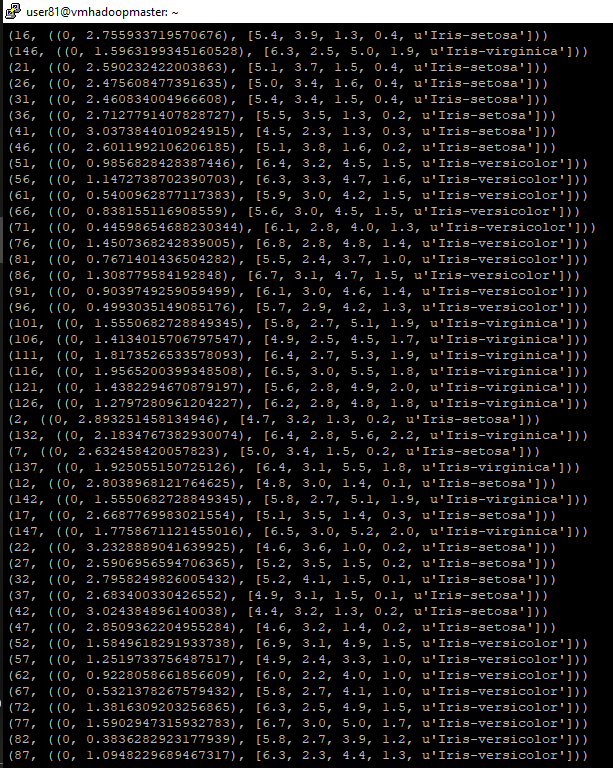
\includegraphics{out2}
\caption{output Part 2
}
\end{figure}\begin{figure}[H]
\centering
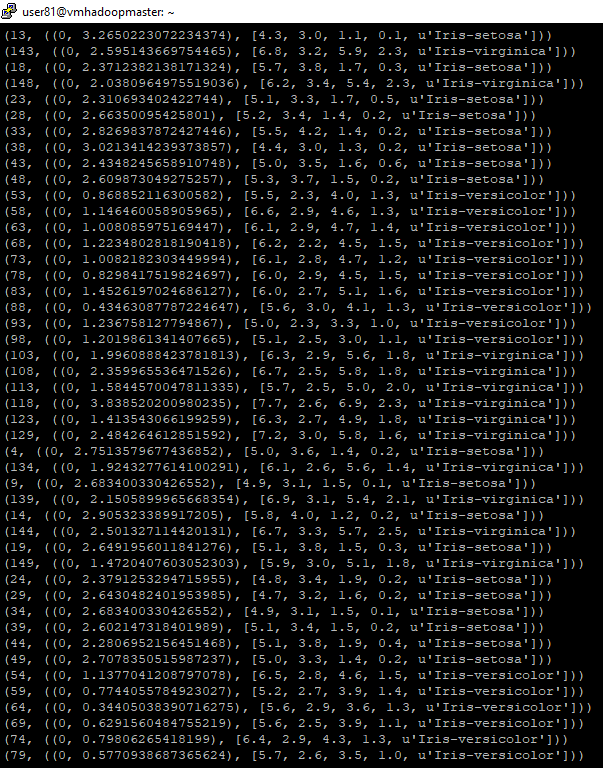
\includegraphics{out3}
\caption{output Part 3
}
\end{figure}\begin{figure}[H]
\centering
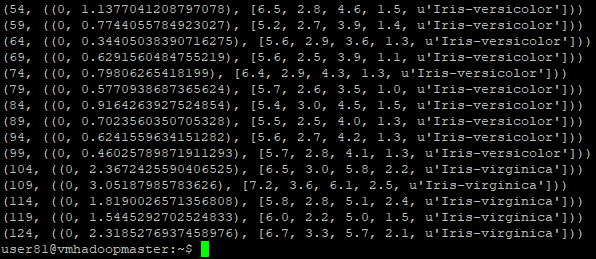
\includegraphics{out4}
\caption{output Part 4
}
\end{figure}
\section{Travaux futurs et perspectives: k-means $++$ avec MapReduce}



Nous consideons maintenant comment reformuler ce dernier algorithmes pour résoudre le problème des k-means$++$ afin qu'ils puissent être appliqués dans un cadre distribué. Plus précisément, nous formulerons une versions distribuées de cet algorithme à l'aide du paradigme \textit{MapReduce}. Nous pensons que cet algorithme peut avoir un grand  potentiel et une grande efficacité sur des datasets à grande échelle.


Rappelons que chaque itération dans l'initialisation de k-means$++$ a deux phases,
\\
 $\bullet$ la première calcule la distance au carré $D (x)$ entre chaque point $x$ et la moyenne la plus proche de $x$, \\
$\bullet$ la seconde échantillonne un membre de $X$ avec probabilité proportionnelle à $D (x)$. Ces deux phases correspondent aux phases \\texttt{Map} et \texttt{Reduce} de notre algorithme MapReduce pour k-means$++$.\v1
La phase Map opère sur chaque point $x$ du Datset. Pour un $x$ donné, nous calculons la distance au carré entre $x$ et chaque moyenne en $M$ et trouver la distance au carré minimale $D (x)$. Nous émettons ensuite une seule valeur $(x; D(x))$,
sans clé. Notre fonction est donc comme suit 
\v1

\no \texttt{kmeansppMap(x):\vskip0.01cm emit $(x,\min_{\mu\in M} ||x-\mu ||^2_2 )$}
\v1
La phase Reduce regroupe toutes les couples emit de la phase \texttt{Map}, car ces émissions n'ont pas de clé. Nous réduisons le premier élément de deux paires de valeurs, en choisissant l'un de ces éléments avec une probabilité proportionnelle au second élément dans chaque paire, et réduire le deuxième élément des paires par sommation. Notre fonction est donc\vskip1cm
\no \texttt{kmeansppReduce$([(x, p), (y, q)])$:  \vskip0.01cm
avec une probabilité $p=(p + q)$: \vskip0.01cm \hskip0.5cm
return $(x, p + q)$  \vskip0.01cm
else:  \vskip0.011cm \hskip0.5cm
return $(y, p + q)$}
\v1
Le MapReduce caractérisé par ces deux fonctions produit une seule valeur de la forme $(x, 1)$ où $x$ est un membre de l'ensemble $X$, et la probabilité qu'un élément particulier $x \in X$ soit renvoyé est proportionnelle à la distance $D (x )$ entre $x$ et la moyenne la plus proche de $M$. Cette valeur $x$ est ensuite ajoutée à $M$ comme moyenne initiale suivante. Comme précédemment, il faut diffuser le nouvel ensemble de moyens $M$ à l'ensemble du cluster entre chaque itération. Nous pouvons écrire l'algorithme entier (désormais appelé k-means$++$) sous la forme suivante: 
\v1\no
=============================================\\
k-means++ MapReduce\\
=============================================
\begin{itemize}
\iti Initialisez $M$, comme suit: $M=\{\mu_1\}$, où $\mu_1$ est choisi uniformément au hasard parmi $X$.
\itii  Appliquez MapReduce kmeansppMap et kmeansppReduce à $X$.
\itiii Ajoutez le point $x$ résultant à $M$.
\itiv Broadcast le nouvel ensemble $M$ sur chaque machine du cluster.
\itv Répétez les étapes (ii) à (iv) au total k-1 fois pour produire $k$ moyennes initiales.
\item[$(vi)$] Appliquez l'algorithme MapReduce k-means standard, initialisé avec ces

\end{itemize}


\section{Conclusion}
Pour ce projet, nous avons examiné le code fournis kmeans-dario-c.py. On a vu comment cet algorithmes de clustering pourraient être implémenté et optimisé.Tout d'abord, nous avons décrit les formulations et analysé leur complexité et leurs coûts. Ensuite, nous avons modifié cet algorithme pour produire une version plus rapide et optimisé. Aussi, on a vu comment on peut construire une extension trés interessante de cet algorithme dans un environnement informatique distribué à l'aide du paradigme de MapReduce. 

\section{Références }
\begin{enumerate}
\item M. Lichman. UCI Machine Learning Repository. University of
California, Irvine, School of Information and Computer Sciences,
http://archive.ics.uci.edu/ml, 2013.
\item David Arthur and Sergei Vassilvitskii. k-means++: The advantages of care-
ful seeding. In Proceedings of the eighteenth annual ACM-SIAM symposium
on Discrete algorithms, pages 1027{1035. Society for Industrial and Applied
Mathematics, 2007.
\item \color{blue} https://github.com/ArsMing276/Kmeans\_Implementation\_with\_Mapreduce
 \color{black}
}\end{enumerate}
\end{document}
